% !TeX encoding = UTF-8
\section{Appendix}
Following are illustrations of reductions of the multigram. Noted that in the following illustrations, we just remove vertices with degree at most one before executing the algorithm instead of vertices with degree at most two, because we want to show how vertices in multigrams are identified.   

\begin{figure}[htbp]
\centering
\begin{minipage}[t]{0.5\textwidth}
\centering
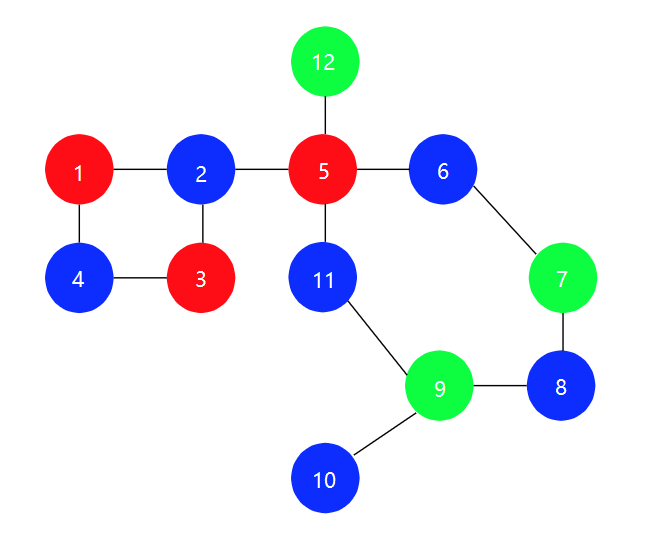
\includegraphics[width=1\textwidth]{figure/1.png}
\caption{\small The input graph}
\end{minipage}
\begin{minipage}[t]{0.48\textwidth}
\centering
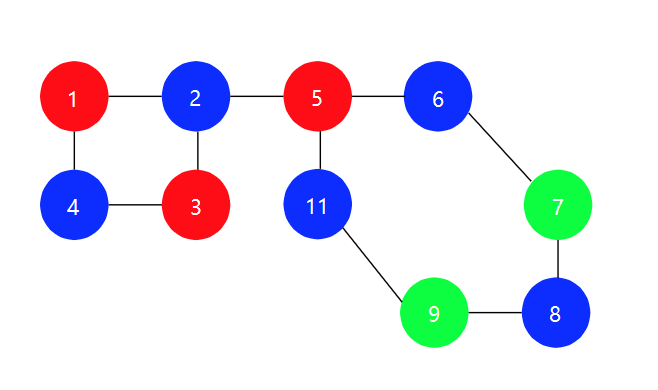
\includegraphics[width=1\textwidth]{figure/2.png}
\caption{\small Remove vertices with degree at most one}
\end{minipage}
\end{figure}

\begin{figure}[htbp]
\centering
\begin{minipage}[t]{0.5\textwidth}
\centering
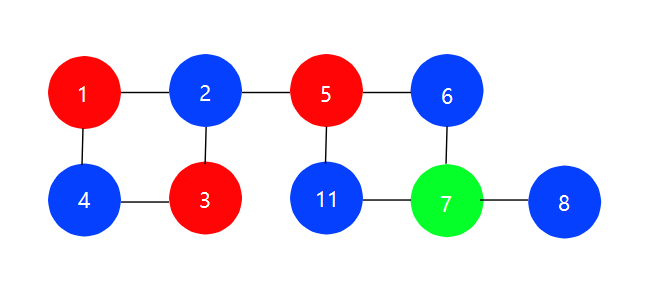
\includegraphics[width=1\textwidth]{figure/3.png}
\caption{\small Identify vertices 7 and 9 which are in a safe hexagram}
\end{minipage}
\begin{minipage}[t]{0.4\textwidth}
\centering
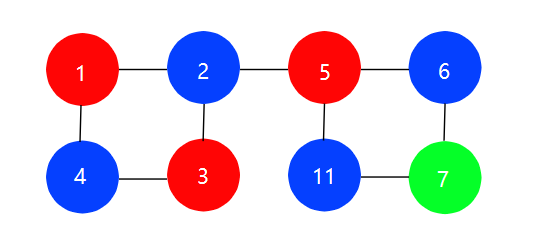
\includegraphics[width=1\textwidth]{figure/4.png}
\caption{\small Remove vertices with degree at most one}
\end{minipage}
\end{figure}

\begin{figure}[htbp]
\centering
\begin{minipage}[t]{0.5\textwidth}
\centering
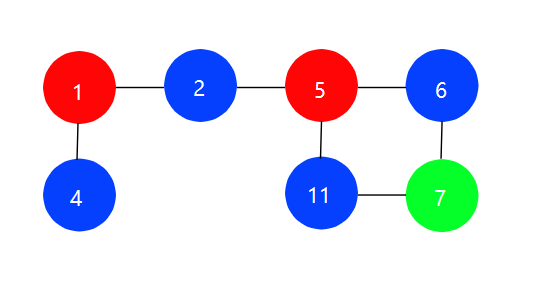
\includegraphics[width=0.8\textwidth]{figure/5.png}
\caption{\small Identify vertices 1 and 3 which are in a safe tetragram}
\end{minipage}
\begin{minipage}[t]{0.48\textwidth}
\centering
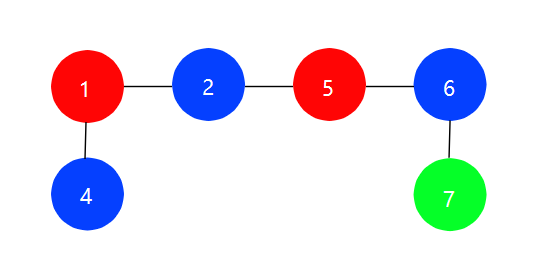
\includegraphics[width=0.8\textwidth]{figure/6.png}
\caption{\small Identify vertices 6 and 11 which are in a safe tetragram}
\end{minipage}
\end{figure}
